% !TeX encoding = UTF-8
% !TeX spellcheck = en_US

\documentclass[
	paper=A4,
	parskip=full,
	chapterprefix=true,
	11pt,
	headings=normal,
	bibliography=totoc,
	listof=totoc,
	titlepage=on,
]{scrreprt}

\usepackage{../../lieb}

\usepackage{feynmp}
\DeclareGraphicsRule{.1}{mps}{*}{}

\graphicspath {{../images/}}

\heads{RWTH Aachen \\ Particlephyics Lab}{T13 \\ Paul Trap}{Lieb | Stettner \\ \today} 
\date{\today}

%\newcommand{\MET}{\ensuremath{{\slashed{E}_\mathrm{T}}}\xspace}

\newcommand{\thirdwidth}{0.32\textwidth}
\newcommand{\halfwidth}{0.48\textwidth}
\newcommand{\fullwidth}{1.0\textwidth}

\setlength\parindent{0pt}
\setlength{\parskip}\medskipamount

\title{Particle Physics Laboratory Class \\ \quad \\ Experiment T13 | Paul Trap }
\author{Jonas Lieb (312136) \\ Jöran Stettner (312169) \\ \\  RWTH Aachen}



\begin{document}

\maketitle

\cleardoublepage

\setcounter{tocdepth}{2}
\tableofcontents

\cleardoublepage

\chapter{Introduction and Theory}

In this laboratory report, the storage of charged particles and a measurement of their specific charge is presented. The experiment consists of a Paul trap, named after its creator Wolfgang Paul, which constrains the movement of a aluminum powder particles to stable trajectories by applying three alternating electrical fields. 

\section{Trapping Particles in Electrical Fields}

Beside the storage of charged particles by B-fields, it is possible to trap particles in electrical fields as well. In a static electrical field of arbitrary shape, the particle will follow the field lines and finally hit the source of the field (e.g. the condensator plate) or diverge (e.g. field of charged sphere). However, by alternating fields it is possible to create on average a minimum of the electrical potential in space. If the frequency of these fields is larger than the movement of the particle, a stable trajectory exists and the particle gets trapped. \\

In a cubic geometry (6 plates, opposing plates at same potential), the following equation of motion holds for all three dimensions. In this so called Mathieu equation, the index $i$ stands for the three spatial components, $\Omega$ is the frequency of the alternating fields, $\xi = \frac{1}{2} \Omega t$ is the normalized time and $a_i, q_i$ are constants depending on the applied voltages and properties of the particle.
\begin{equation}
\label{eq:mathieu}
\left(a_i+q_i \cos(2 \xi)\right) x_i + \frac{d^2x_i}{d\xi^2} = 0
\end{equation}

The full solution of this equation is discussed elsewhere (e.g. in the lab manual\cite{Lab_manual}), the following aspects are important for the conducted experiment.

\subsection{Stability of the Particle Trajectories}
The exact solution for the particle trajectories can be expressed in an infinite series. However, the tracks are only finite under certain conditions. Depending on the applied alternating field $U_i$ and the constant field $U_{G}$ (same potential on both plates), the constants $a$ and $q$ change. The constants in x-direction are given in equation \ref{eq:a} and \ref{eq:q}, where $K$ is a geometry factor of the plates, $m$ the mass of the particle, $q$ the charge of the particle and $r_0$ the distance of the plates to the center.
\begin{equation}
	\label{eq:a}
	a_x=\frac{16 K q}{3 \Omega^2 m r_0^2} U_{G,x}
\end{equation}
\begin{equation}
	\label{eq:q}
	q_x= \frac{-4 K q}{ \Omega^2 m r_0^2} U_{x}
\end{equation}

For stable trajectories, the voltages have to be adjusted such that the following equation holds\cite{Lab_manual}:
\begin{equation}
 \beta_x  = \sqrt{a_x+\frac{q_x^2}{2}}  \in (0,1)
\end{equation}
Additionally, air friction helps to stabilize the particle tracks since it damps the motion (Stoke's term in the Mathieu equations leads to weaker conditions). 

\subsection{Influence of an Additional Force in z-Direction}
Instead of applying an additional potential to both x-plates, it is also possible to apply an additional static electrical field in z-direction (homogeneous, pointing upwards, different potential on the plates). The idea is to compensate the gravitational force which acts on the particle. If considered in the Mathieu equations, a net force in z-direction does not change the shape of the particle tracks but shifts the center of the trajectories. However, if the applied field compensates the gravitational force, there is no shift of the particles and the particle tracks becomes independent of the applied alternating voltage $U_z$ \cite{Lab_manual}.

\subsection{Influence of an Additional Alternating Field in x-Direction}

As a third option, the influence of an additional alternating field in x-direction is discussed. While the alternating fields $U_i$ have same potential on opposing plates, the field $U_W$ acts homogeneously in x-direction (different potential on opposing plates). The additional term in the Mathieu equation leads to modified trajectories: The particle shakes back and forth and by changing the driving frequency of the field $U_W$ also resonances can be observed (forced,damped harmonic oscillator with damping constant $k_L$ from the Stoke's term describing air friction):
\begin{equation}
\omega_W^{res} = \frac{\Omega}{2} \sqrt{\beta_x^2 - 2 k_L^2}
\end{equation}



\chapter{Experimental Setup}

The trap consists basically of 6 copper rings and a high voltage source, see figure \ref{fig:trap}. The rings are arranged in a cubic geometry: Each two rings facing each other lie on the same potential. The amplitude of the voltages $U_x$,$U_y$ and $U_z$ can be adjusted individually, but the phase between them remains $120^\circ$. Additionally, a lamp and a camera are used to illuminate and observe the trapped particles inside the trap (not visible on the picture). To inject a few particles of aluminum powder, a syringe is installed below the trap. By pressing it, the particles are pushed upwards and become charged by the friction with the surrounding material of the syringe or air. \\

\begin{figure}
	\centering
	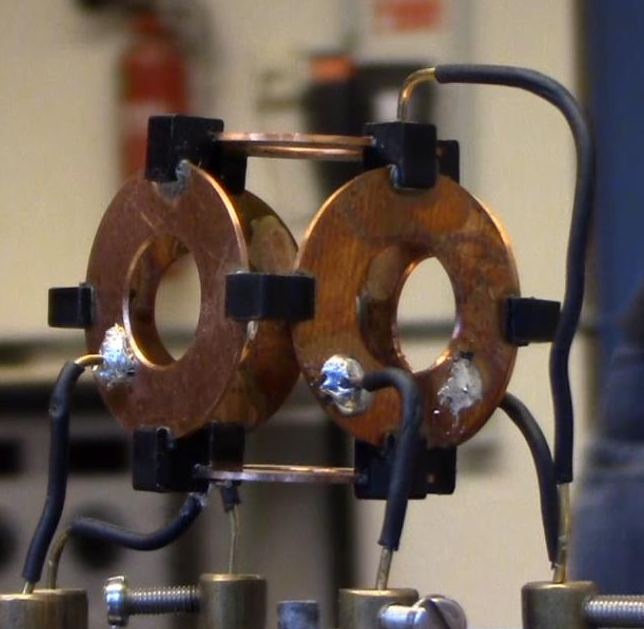
\includegraphics[width=\halfwidth]{capture_20150916_124003_cut}
	\caption{Picture of the Paul Trap during installation. The 6 copper rings are connected to a three phase high voltage supply.}
	\label{fig:trap}
\end{figure}

Furthermore, three additional voltages can be applied to some rings of the trap:
\begin{itemize}
	\item An additional direct voltage to the two rings in x-direction: $U_{G,x}$ (same potential on both x-rings)
	\item A direct voltage in z-direction creating a constant electrical field in upwards in z-direction (different potential on the two z-rings): $U_{G,z}$
	\item An overlayed alternating voltage on both x-rings (different potential) creating an alternating field in x-direction: $U_W$
\end{itemize}





\chapter{Conduction and Analysis}
\label{ch:analysis}
In the following chapter, the conducted experiments and their results are reported. Each measurement is repeated in a low pressure environment to investigate the influence of air friction on the trapped particles. Since the particle trajectories are much more instable without air friction, the low pressure cylinder is not evacuated to the lowest limit of the vacuum pump ($p \approx \SI{5}{\micro \bar}$), but operated once at $p = \SI{300}{\milli \bar}$ and once at $p = \SI{150}{\milli \bar}$. \\
Each conducted measurements yields a value of the specific charge $\frac{q}{m}$ which is different for the aluminum particles because their size and their aquired charge differ. To compare the different methods, the measurements are conducted in a series with the same trapped particle.\\
AS discussed in chapter \ref{ch:systematics}, the output of the high voltage source does not match its adjusted values. The following correction factors are therefore applied to all adjusted voltages and will be justified later:

\begin{table}[htbp]
	\centering
	\begin{tabular}{ 
			l
			l
		}
		\toprule
		Voltage & Correction Factor \\ 
		\midrule
		$U_x$ & $0.78 \pm 0.02$  \\
		$U_y$ & $0.76 \pm 0.03$ \\
		$U_z$ & $0.81 \pm 0.03$ \\
		$U_K$ and $U'$ & $0.61 \pm 0.01$ \\
		$U_W$ & $0.17 \pm 0.03$ \\
		
		\bottomrule
	\end{tabular}
	\caption{Correction factors to compensate for the wrong mismatching output of the voltage supply. The determination of these factors is described in chapter \ref{ch:systematics}.}
	\label{tbl:corr_factors}
\end{table}


\section{Measurement I - Stability of the Trajectories}
\section{Measurement II - Application of an Additional Field in z-Direction}
\section{Measurement III - Resonance Study}

\chapter{Systematic Uncertainties}
\label{ch:systematics}
\section{High Voltage Source}
\subsection{Mismatch of the Internal Voltage Measurement}
The high voltage source displays the adjusted voltage, see figure \ref{fig:voltagesource}. However, a cross-check measurement with a multimeter shows discrepancies for all voltages of the source. To account for this, correction factors have been introduced in chapter \ref{ch:analysis}. They were determined by measuring four values and comparing them to the displayed values. The ratio of these values is averaged and the standard deviation is propagated through all analysis steps as a systematic uncertainty. TODO: Wirklich? Oder negligible ? 
\subsection{Fluctuations of the Voltage Source}

\chapter{Comparison of Results}


\cleardoublepage

\bibliographystyle{utphys}
\bibliography{T13_bib}{}

\end{document}


